\chapter{JFET CHARACTERISTICS}

\subsection*{AIM}
\paragraph{}To design and implement a circuit for simulating the drain and transfer characteristics of a JFET.

\subsection*{DESIGN AND CIRCUIT DIAGRAM}
\paragraph{}

Inorder to draw the JFET characteristics, we have to use a DC source of voltage which may be varied during simulation. The JFET in the circuit should be associated with a coresponding `JFET model' during  simulations. The resulting circuit diagram is shown in the Figure \ref{JFETckt}.
\begin{figure}[h]
\centering
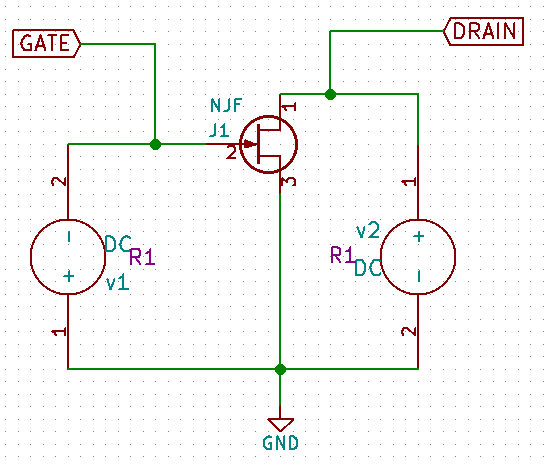
\includegraphics[width=0.8\textwidth]{JFETckt.png}
\caption{Schematic diagram for JFET characteristics}
\label{JFETckt}
\end{figure}

Drain charcteristics is a plot between the drain current and drain to source voltage keeping the gate voltage constant. Transfer charcteristics is a plot between the drain current and gate to source voltage keeping the drain voltage constant.

\subsection*{PROCEDURE}

\subsubsection{Launch eSim}

\paragraph{}
 Launching eSim will take you to the dialog box which asks for the default workspace. Browse the folders and set the wokspace location. It will finally end up in the eSim window %shown in Figure \ref{LaunchWindow}.
%\begin{figure}[h]
%\centering
%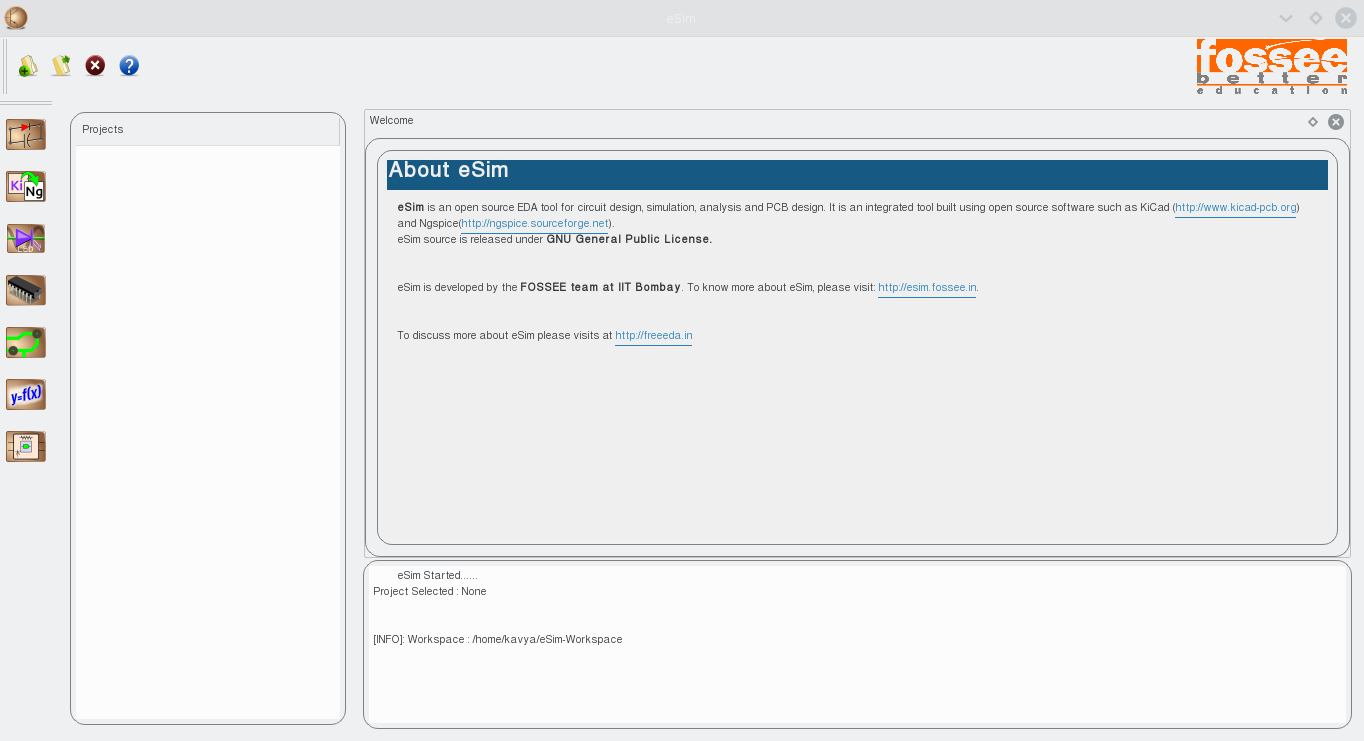
\includegraphics[width=0.8\textwidth]{LaunchWindow.png}
%\caption{Launching eSim will take you to this window}
%\label{LaunchWindow}
%\end{figure}

\subsubsection{Create a New Project}

\paragraph{ } The new project is created by clicking the New icon on the
menubar. The name of the project is given in the pop up window.% as shown in Figure.\ref{newproject}.
%\begin{figure}[h]
%\centering
%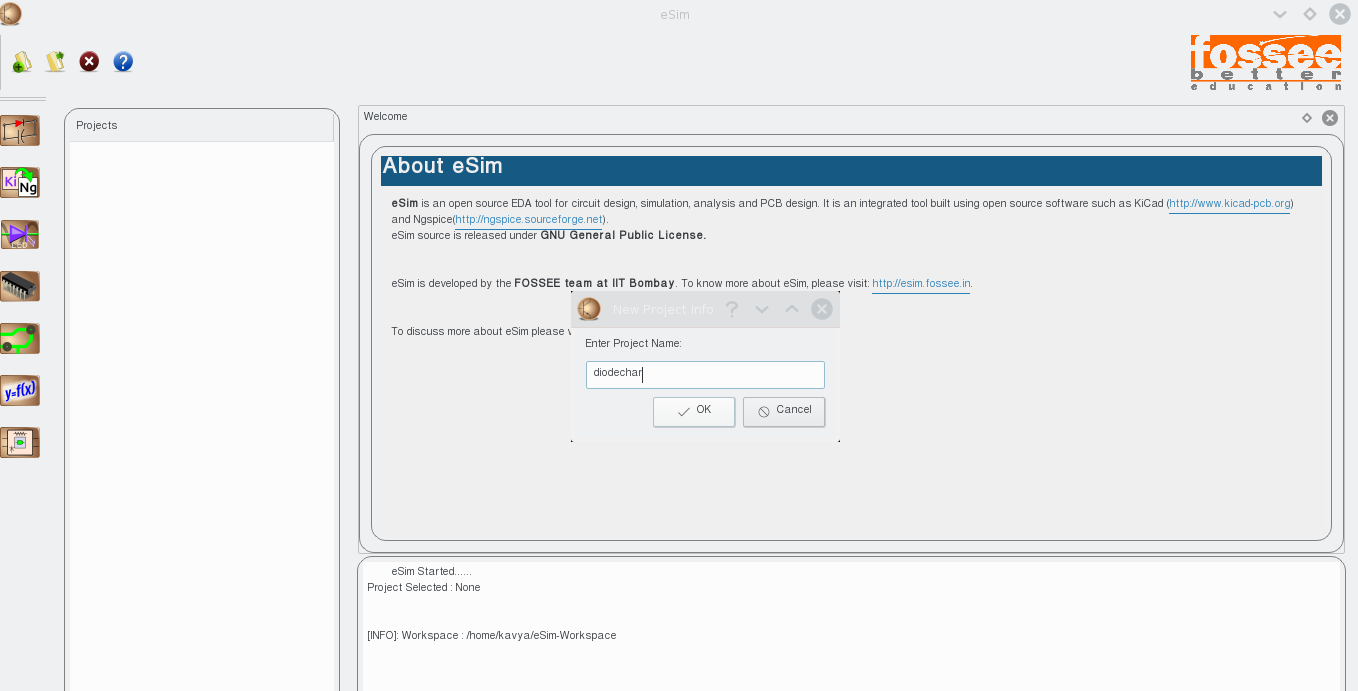
\includegraphics[width=\textwidth]{newproject.png}
%\caption{Creating new project}
%\label{newproject}
%\end{figure}

\subsubsection{Create the Schematic}

\paragraph{}  To create the schematic, click the very first icon of the
left toolbar.% as shown in the Figure \ref{newschematic} .
This will open KiCad Eeschema.


%\begin{figure}[h]
%\centering
%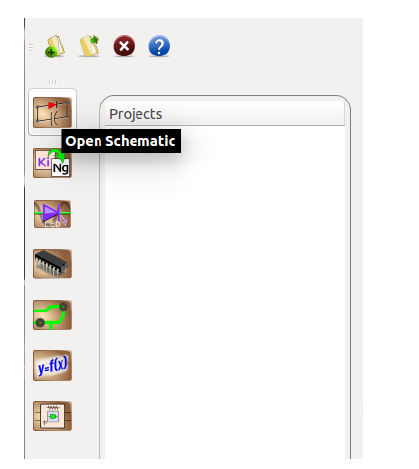
\includegraphics[width=0.5\textwidth, height=6cm]{newschematic.png}
%\caption{Creating new schematic diagram}
%\label{newschematic}
%\end{figure}

To create a schematic in KiCad, we need to place the required components. %See Figure \ref{kicad}

%\begin{figure}[h]
%\centering
%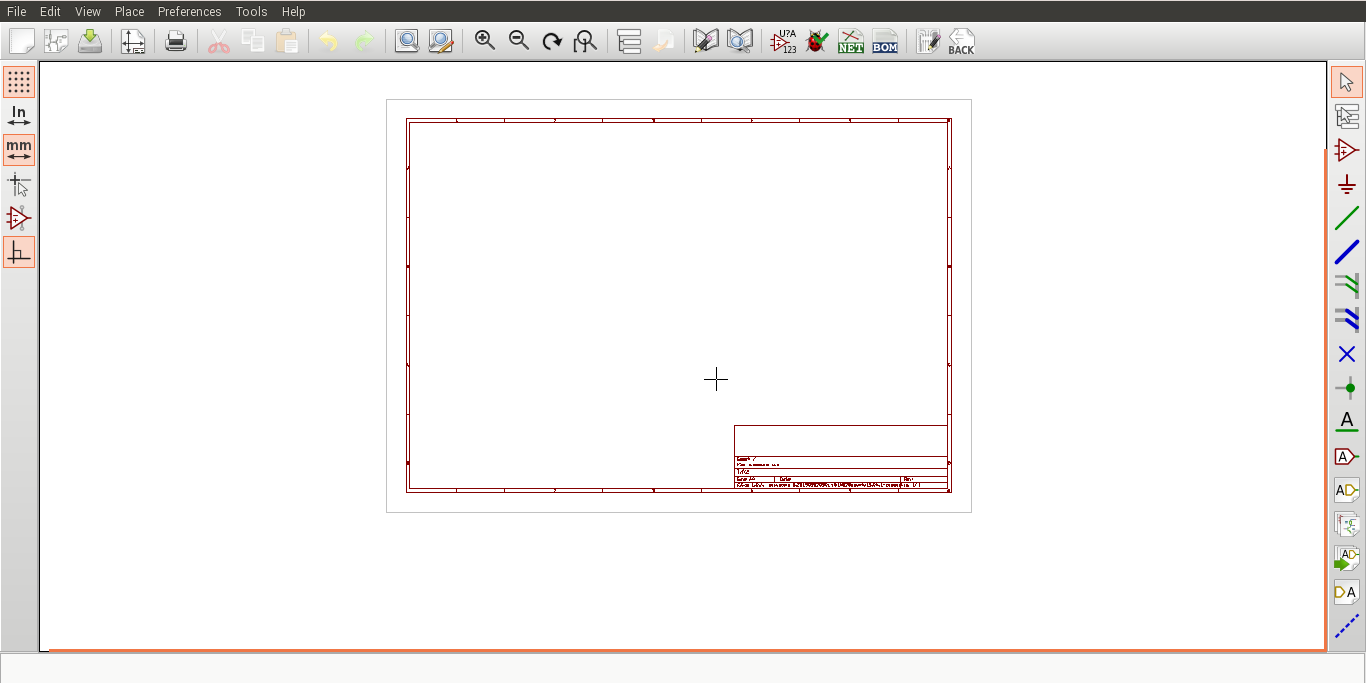
\includegraphics[width=0.5\textwidth, height=6cm]{kicad.png}
%\caption{The Kicad Eeschema page}
%\label{kicad}
%\end{figure}

 Clicking on the icon on the right toolbar opens the component library. After all the required components of the circuit are placed, wiring is
done using the Place Wire option. %as shown in the Figure \ref{placewire}.
 Scroll up and down for zooming in and out.


%\begin{figure}
%\begin{minipage}{.5\textwidth}
%  \centering
%  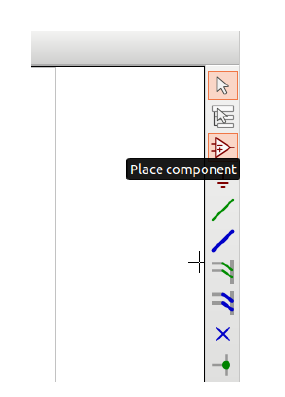
\includegraphics[width=\linewidth]{placecomponent.png}
%  \caption{Place component icon}
%  \label{placecomponent}
%\end{minipage}%
%\begin{minipage}{.5\textwidth}
%  \centering
%  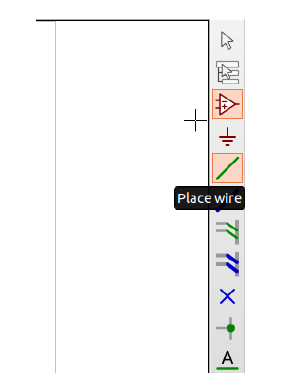
\includegraphics[width=\linewidth]{placewire.png}
%  \caption{Place wire icon}
%  \label{placewire}
%\end{minipage}
%\end{figure}


\paragraph{Placing the Components:} Normally all the components availbale in eSim can be chosen by left mouse click in the grid. The components are listed in different libraries. %See Figure \ref{librarylist}.

%\begin{figure}[h]
%\centering
%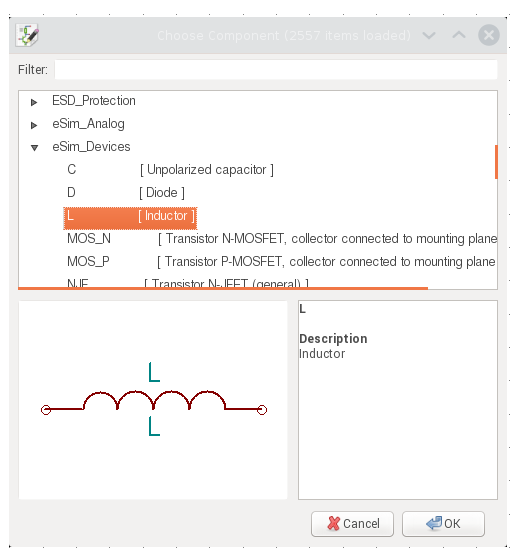
\includegraphics[width=0.5\textwidth, height=4cm]{librarylist.png}
%\caption{The Kicad Libraries of components}
%\label{librarylist}
%\end{figure}

\begin{itemize}
\item
Choose DC sources from eSim\_Sources
\item
Choose NJF from eSim\_Devices
\item
Choose GND from power
\end{itemize}

%Select the resistor and edit its component value to 1k as shown in Figure \ref{editvalue}.

%\begin{figure}[h]
%\centering
%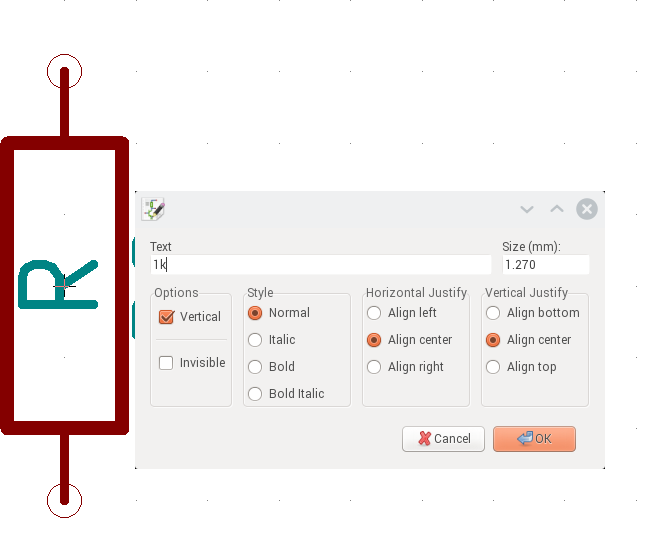
\includegraphics[width=0.5\textwidth, height=6cm]{editvalue.png}
%\caption{Editing the value field of component R}
%\label{editvalue}
%\end{figure}

Wire the components to get the circuit. A global labels `GATE' and `DRAIN' hav been added to identify those nodes whose voltage will be later recorded and plotted.

\paragraph{Annotating the circuit:} Once the schematic diagram is completed, annotate it so that the `question marks' associated with the components are converted to meaningful numbers automatically.For that choose annotate button from the top toolbar%(See Figure \ref{toptoolbar} 
and in the subsequenct dialogue boxes appearing click ok and finally close. See Figure \ref{annotation7}.

%\begin{figure}[h]
%\centering
%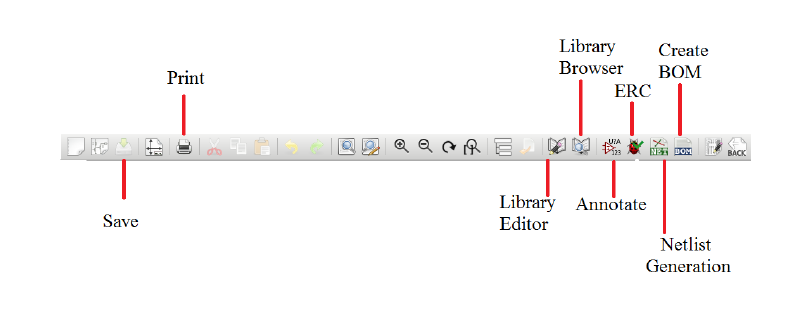
\includegraphics[width=\textwidth, height=4cm]{toptoolbar.png}
%\caption{Choose annotate from the toop tool bar}
%\label{toptoolbar}
%\end{figure}



Now we have the circuit diagram as shown in Figure \ref{JFETckt}.


\paragraph{Note:} If some libraries are found missing, you can add them from the `Preferences` menu by following the procedure: 

\begin{enumerate}
\item
Choose `Component Libraries' from Preferences menu.

\item
Click on the Add button on the top right side of the window.

\item
Choose the required libraries from `user/share/kicad/library' and click OK button

\end{enumerate}

\subsubsection{Create Netlist}

\paragraph{}To simulate the circuit that has been created in the previous section, we need to generate
its netlist. Netlist is a list of components in the schematic along with their connection
information. To do so, click on the Generate netlist tool from the top toolbar. Click on
spice from the window that opens up. Check the option Default Format. Then click
on Generate. Save the netlist. This will be a .cir file. Do
not change the directory while saving.See Figure \ref{createnetlist7}.
 Now the netlist is ready to be simulated. 
\begin{figure}
\begin{minipage}{.5\textwidth}
  \centering
  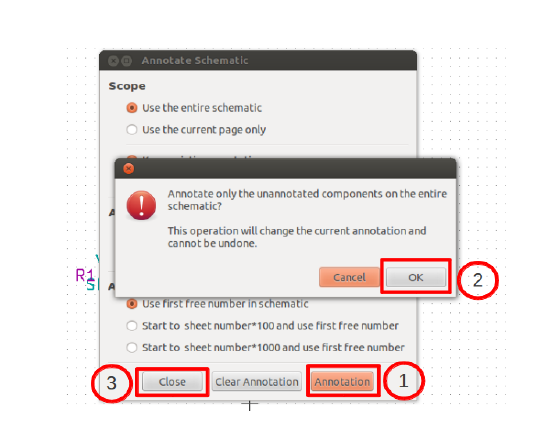
\includegraphics[width=\linewidth]{annotation.png}
  \caption{Annotation}
  \label{annotation7}
\end{minipage}%
\begin{minipage}{.5\textwidth}
  \centering
  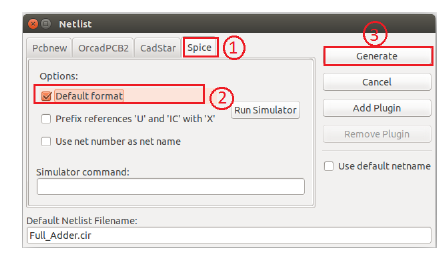
\includegraphics[width=\linewidth]{createnetlist.png}
  \caption{Netlist Generation}
  \label{createnetlist7}
\end{minipage}
\end{figure}

\subsubsection{KiCad to Ngspice conversion}

\paragraph{} To convert KiCad netlist of JFET circuit to NgSpice
compatible netlist click on KiCad to Ngspice icon as shown in Figure \ref{kcd2spice7}.  Now you can choose the type of analysis, source details, device models ngspice models and subcircuit models.


\begin{figure}[h]
\centering
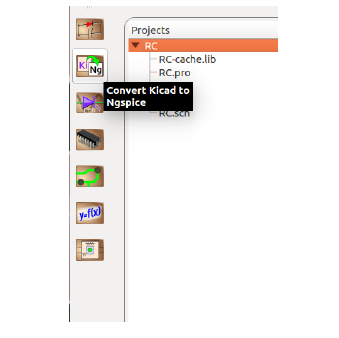
\includegraphics[width=0.5\textwidth, height=4cm]{kcd2spice.png}
\caption{Choose Kicad to Ngspice tool}
\label{kcd2spice7}
\end{figure}


\paragraph{Analysis:}Choose DC analysis type. On the same netlist you can simulate the drain characteristics as well as transfer charcteristics. Choose the values of two DC sources, V1 and V2 in the netlist properly as described below. Follow the procedures for drain characteristics first. After obtaining the required plots do the procedures for the transfer characteristics and obtain the required charcteristics curves.

\begin{itemize}
\item 
\textbf{Drain Charcteristics:} Give the values of DC variables as shown in Figure \ref{analysisdrain}. Enter the name of your DC source \textbf{V2} and let its value be varied from 0V to 30V with a step of 0.1 V.


\item
 \textbf{Transfer Charcteristics:} Give the values of DC variables as shown in Figure \ref{analysistransfer}. Enter the name of your DC source \textbf{V1} and let its value be varied from 0V to 4V with a step of 0.1 V.


\end{itemize}

\begin{figure}[h]
\centering
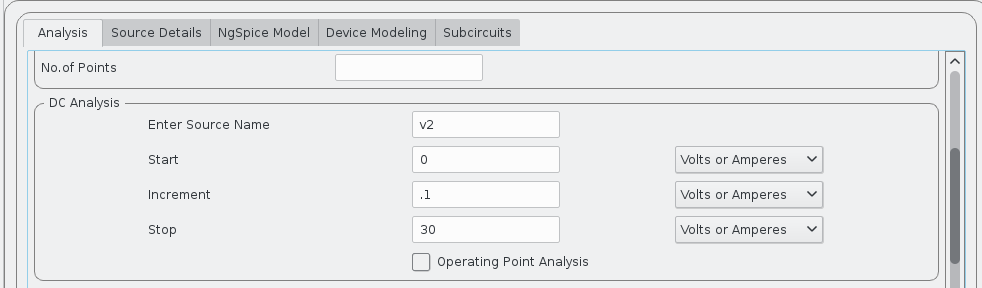
\includegraphics[width=\textwidth, height=4cm]{analysisdrain.png}
\caption{Choose DC analysis type and enter the values of V2}
\label{analysisdrain}
\end{figure}

\begin{figure}[h]
\centering
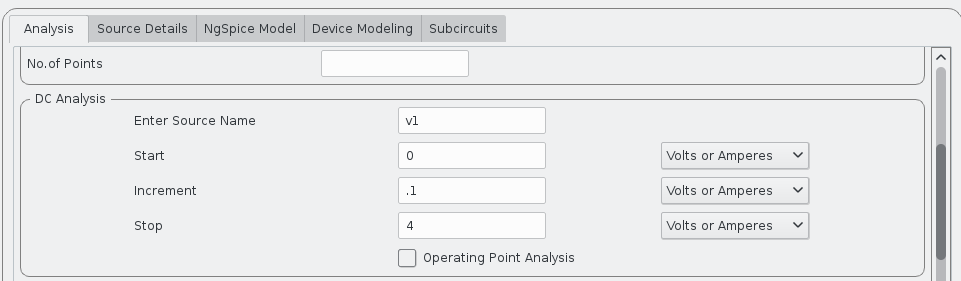
\includegraphics[width=\textwidth, height=4cm]{analysistransfer.png}
\caption{Choose DC analysis type and enter the values of V1}
\label{analysistransfer}
\end{figure}
\paragraph{Source Details:} 
\begin{itemize}
\item \textbf{Drain Charcteristics:} Give the value of DC variables as shown in Figure \ref{dcsourcedrain}. Leave the column of V2 blank. Give the value of V1 as 0V, which is the gate voltage. (You may repeat the experiment by varying the gate voltage as V1=1V, V1=2V etc.)
\begin{figure}[h]
\centering
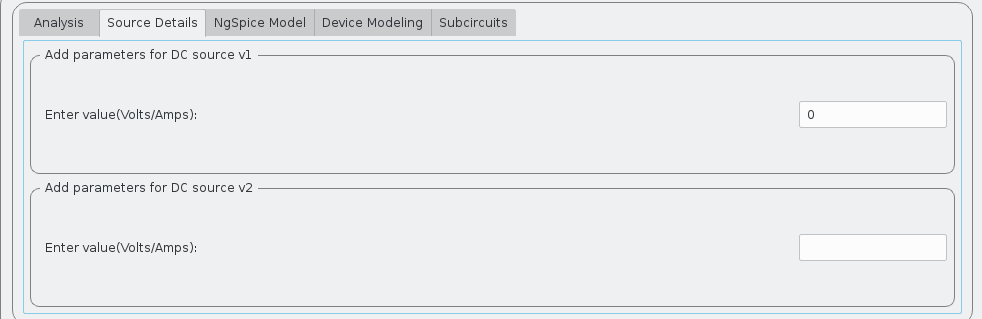
\includegraphics[width=\textwidth, height=4cm]{dcsourcedrain.png}
\caption{Enter the details of fixed source V1}
\label{dcsourcedrain}
\end{figure}

\item \textbf{Transfer Charcteristics:} Give the value of DC variables as shown in Figure \ref{dcsourcetransfer}. Leave the column of V1 blank. Give the value of V2 as 3V, which is the drain voltage. 
\begin{figure}[h]
\centering
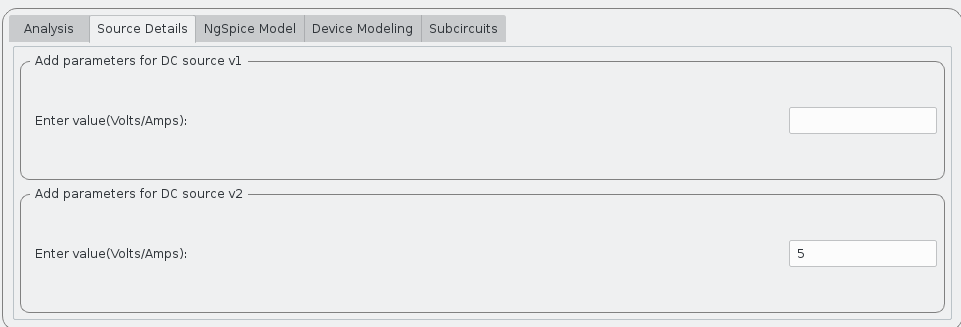
\includegraphics[width=\textwidth, height=4cm]{dcsourcetransfer.png}
\caption{Enter the details of fixed source V2}
\label{dcsourcetransfer}
\end{figure}

\end{itemize}

\paragraph{Ngspice Model:} No Ngspice model to be given.

\paragraph{Device Model:} The JFET is a device whose model details must be given for simulation. Let us choose the generic N-chnnel JFET model availabe in the eSim model library. Browse it from \texttt{/opt/eSim/src/deviceModelLibrary/JFET/NJF.lib}. See Figure \ref{JFETmodel}.
\begin{figure}[h]
\centering
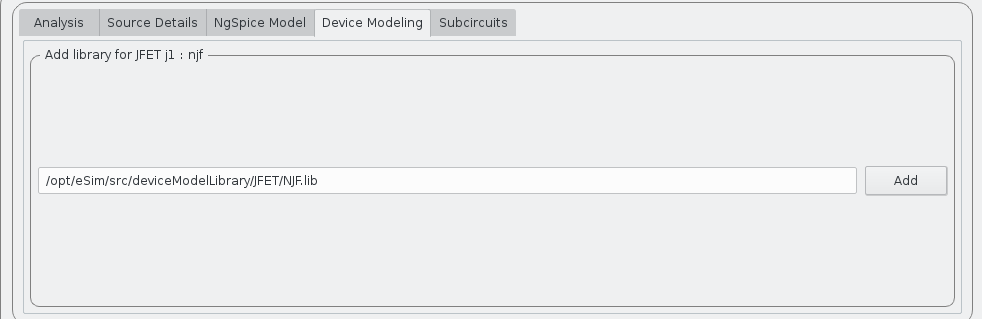
\includegraphics[width=\textwidth, height=6cm]{JFETmodel.png}
\caption{Choose the required JFET model}
\label{JFETmodel}
\end{figure}

\paragraph{Subcircuits:} No subcircuits to be given.

\paragraph{}
 Once these details are provided click on convert button. %See Figure \ref{diodemodel}. 
Now you are ready to see the simulation results.

\subsubsection{Simulate} To run Ngspice simulation click the simulation icon in the left tool bar. It will open up two windows - ngspice plotting window and python plotting window. Inorder to plot the JFET characteristics let us use the commands in ngspice plotting window. We need to plot the drain charcteristics as well as transfer characteristics.

\paragraph{Drain Characteritics:} In the ngspice plotting window, type the following command:

\texttt{plot -i(v2) vs v(drain)}

This would pop up the drain characteristics of the JFET as defined in the JFET model NJF.lib. For a differnt device model the characteristics would be slightly different.

The resultant characteristics is shown in the Figure \ref{JFETdrain0} and \ref{JFETdrain1}.
\begin{figure}[h]
\centering
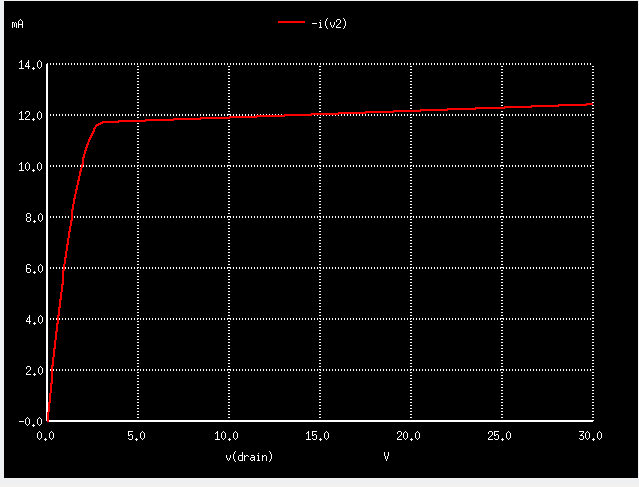
\includegraphics[width=12cm, height=6cm]{JFETdrain0.png}
\caption{The drain characteristics of JFET with gate voltage =0V }
\label{JFETdrain0}
\end{figure}
\begin{figure}[h]
\centering
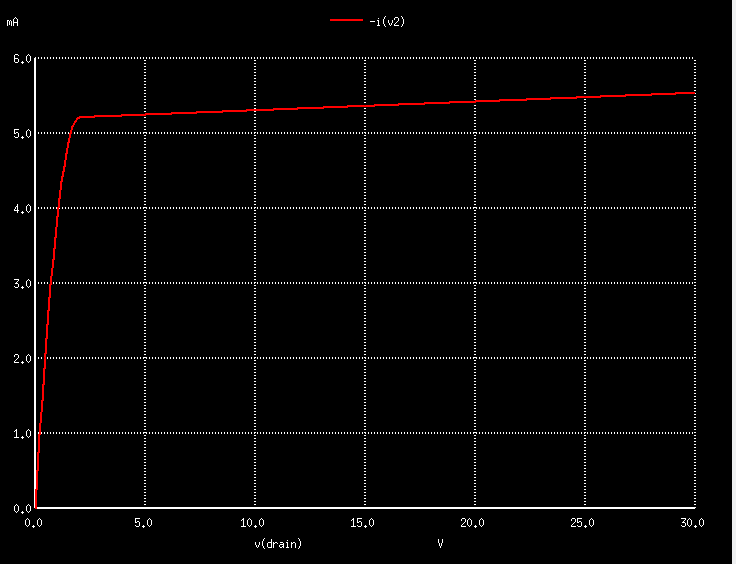
\includegraphics[width=12cm, height=6cm]{JFETdrain1.png}
\caption{The drain characteristics of JFET with gate voltage =1V }
\label{JFETdrain1}
\end{figure}

\paragraph{Transfer Characteritics:} In the ngspice plotting window, type the following command:

\texttt{plot -i(v2) vs v(gate)}

This would pop up the transfer characteristics of the JFET as defined in the JFET model NJF.lib. For a differnt device model the characteristics would be slightly different.

The resultant characteristics is shown in the Figure \ref{JFETtransfer}.


\begin{figure}[h]
\centering
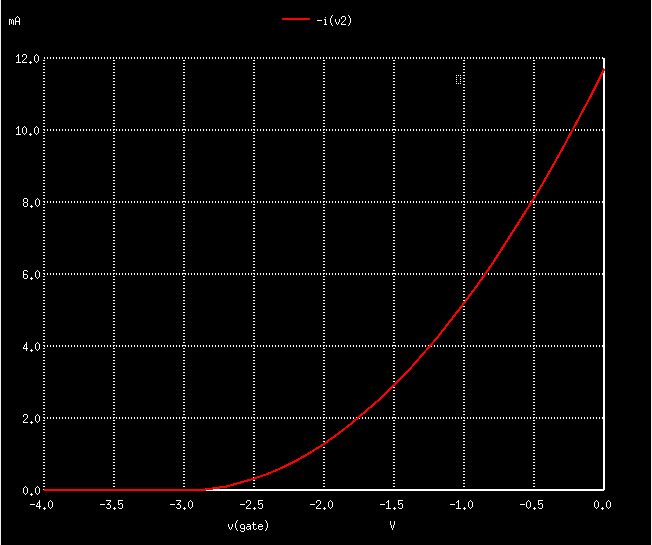
\includegraphics[width=12cm, height=6cm]{JFETtransfer.png}
\caption{The transfer characteristics of JFET with drain voltage =3V }
\label{JFETtransfer}
\end{figure}


\section*{RESULT}
The circuit for plotting the charateristics of JFET was implemented and simulated.


